\documentclass[12pt]{article}

\usepackage{amsthm}
\usepackage{amsmath}
\usepackage{graphicx}
\graphicspath{ {images/}{figs/} }
\usepackage{listings}
\lstset{
  basicstyle=\ttfamily,
  columns=fullflexible,
  frame=single,
  breaklines=true,
}

\theoremstyle{definition}
\newtheorem{definition}{Definition}

\title{{\small{Machine Learning and Algorithms for Data Mining} \\
Assessment 2\footnote{Word count: 2467 --- Computed using TexCount}} \\
\textit{Analysis of graph-structured data}}
\author{Sebastian Borgeaud --- spb61@cam.ac.uk}

\begin{document}
\maketitle

\begin{abstract}
	In this report I explore the efficiency of various algorithms on the task of transductive classification on a graph. In particular, I focus on the cora dataset, consisting of 2078 scientific publications each classified into one of seven classes. Each publication is described by a bag-of-word vector for a vocabulary of 1433 unique words. The edges in the graph represent citations (REFERENCE).
	\end{abstract}

\section{Main contributions, Key Concepts and Ideas}
\subsection{Introduction}
Many real world datasets occur naturally in the form of graphs, for example protein-protein interaction networks in biology, social networks in social sciences and relational databases to name just a few examples from different fields. (CITATIONS) In this report I focus on the problem of node classification in the transductive setting. At training time, the entire structure of the network is known but only few nodes are labelled. At test time, we wish to infer the labels of some or all of the remaining nodes. This differs from supervised learning in two ways: i) the data points (the nodes) are connected to each other and ii) the features of the nodes that will be classified at test time are known in advance, i.e. the graph is known at test time. 
Instead, the problem can be seen as a graph-based semi-supervised learning problem, where the label information is smoothed over the graph via some form of explicit graph-based regularisation. For example, we could make the assumption that adjacent nodes are more likely to have the same class label and incorporate this in the loss
\begin{equation}
	\mathcal{L} = \mathcal{L}_0 + \lambda \mathcal{L}_{\mathit{reg}}
\end{equation}
where $\mathcal{L}_0$ is some supervised loss w.r.t to labeled nodes and $\mathcal{L}_{\mathit{reg}}$ is a graph Laplacian regularisation term using the made assumption.

\subsection{Dataset}
I focus on the cora dataset, consisting of 2078 machine learning publications, each representing a node in the graph (REFERENCE). Each publication is classified into one of seven classes: `Case Based', `Genetic Algorithms', `Neural Networks', `Probabilistic Methods', `Reinforcement Learning', `Rule Learning' or `Theory'. Each publication has a binary bag-of-word feature vector for a vocabulary of 1433 unique words. The edges are directed (WRONG, adj.transpose == adj) and represent citations, where an edge $\mathit{pub_1} \to \mathit{pub_2}$ means that publication $\mathit{pub_2}$ is cited in publication $\mathit{pub_1}$. The papers were selected in such a way that every paper cites or is cited by at least one other paper.

In particular, I use the data split introduced by Kipf and Welling \cite{kipf2017semi}. At training time the label of only 140 nodes is given (about 6.7\%). A further 500 node labels are given as validation data. We wish to infer the label of 1000 nodes not contained in either the test or validation set. Furthermore, the edge orientations are ignored by constructing a symmetric adjacency matrix.

The distribution of node degrees is plotted in figures \ref{fig/node_degrees} and \ref{fig/node_degrees_truncated}. Most nodes have few outgoing edges, with 59.9\% of the nodes having 3 outgoing edges or less and over 96.5\% having 10 or fewer. There seems to be one extreme outlier publication making 168 citations, whereas the second most citing paper makes only 78 citations.

\begin{figure}[h]
	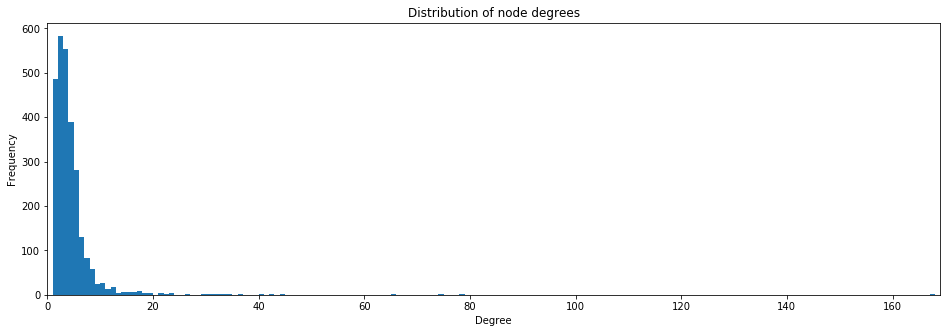
\includegraphics[width=1.0\textwidth]{node_degrees}
	\centering
	\caption{Distribution of node degrees in Cora dataset}
	\label{fig/node_degrees}
\end{figure}

\begin{figure}[h]
	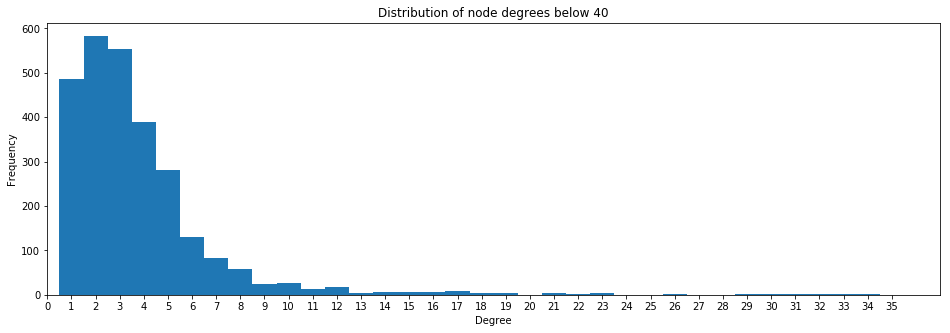
\includegraphics[width=1.0\textwidth]{node_degrees_truncated}
	\centering
	\caption{Distribution of node degrees for nodes with degree below 40. This includes 2701 of the 2708 publications, or above 99.7\% of the nodes.}
	\label{fig/node_degrees_truncated}
\end{figure}

\section{Methods}
\subsection{SVM on features alone}
First, I create a simple baseline model by training an SVM on the features of the nodes only, i.e.\ the bag-of-words vectors of the publications. This approach ignores the structure of the graph entirely and is therefore an instance of a supervised learning problem. In particular, given a bag-of-word representation of a publication we wish to infer its publication type. 

I trained the SVM on the training instances of the dataset. The trained model is then used to predict the class labels of the test publications. The model hyper-parameters are optimised using the validation data set. For the kernel I considered both a linear and a radial basis function. The 
\subsection{SVM with neighbouring features}
\subsection{Graph Convolutional Network}
\subsection{Graph Attention Networks}

\section{Results \& analysis}

\section{Conclusion}

\bibliography{bib}
\bibliographystyle{unsrt}


\end{document}